\documentclass[a4paper,draft]{scrbook}
\usepackage{a4wide,amsmath}
\usepackage[final]{graphicx}
\usepackage[square,numbers]{natbib}
\usepackage[draft=false]{hyperref}  %% need this for links and references in the document
\usepackage{array}     %% need this for more table formating (m{} and p{})
\usepackage{url}       %% support for URLs
\usepackage{float}     %% required for extra float placement
\usepackage{xcolor}
\usepackage{placeins}
\usepackage{subfig}
\usepackage{lscape}    %% landscape figures
\usepackage{todonotes}
\usepackage{color}
\usepackage[figuresright]{rotating}
\usepackage{minted}    %% excellent source code formating
\usepackage{tikz}

\usetikzlibrary{trees,shapes.geometric,positioning}

\definecolor[named]{desycyan}{rgb}{0,0.648,0.918}
\definecolor[named]{desyorange}{rgb}{0.945,0.555,0}
\definecolor[named]{desygray}{rgb}{0.465,0.465,0.465}
\definecolor[named]{desywhite}{rgb}{1,1,1}

\hypersetup{pdftitle={libpniio API review 2013 },
        	pdfborder=0 0 0,
	    	colorlinks=false}

\setcapindent{0em}

\title{{\Huge{\tt libpniio} Users Guide}}
\author{Eugen Wintersberger}

\newcommand{\libpnicore}{\texttt{libpnicore}}
\newcommand{\libpniio}{\texttt{libpniio}}
\newcommand{\sdarray}{\texttt{static\_array}}
\newcommand{\darray}{\texttt{dynamic\_array}}
\newcommand{\farray}{\texttt{fixed\_dim\_array}}
\newcommand{\mdarray}{\texttt{mdarray}}
\newcommand{\arrayview}{\texttt{array\_view}}
\newcommand{\arrayerasure}{\texttt{array}}
\newcommand{\numarray}{\texttt{numeric\_array}}
\newcommand{\cmake}{\texttt{cmake}}
\newcommand{\pkgconfig}{\texttt{pkg-config}}
\newcommand{\gcc}{\texttt{gcc}}
\newcommand{\nxfield}{\texttt{nxfield}}
\newcommand{\nxobject}{\texttt{nxobject}}
\newcommand{\nxgroup}{\texttt{nxgroup}}
\newcommand{\nxattribute}{\texttt{nxattribute}}
\newcommand{\nxpath}{\texttt{nxpath}}
\newcommand{\cpp}[1]{\texttt{#1}}

%\bibliographystyle{plainnat}

\newminted{cpp}{fontsize=\small,frame=lines}

\begin{document}
\maketitle
\tableofcontents
\listoftodos

\chapter{Introduction}\label{chapter:introduction}
\input{tex/introduction.tex}
\FloatBarrier

\chapter{Installation}\label{chapter:installation}
%%% describe the installation procedure


\section{Install precompiled packages}

\section{Install from sources}

\subsection{Running tests}

In order to run the tests use 
\begin{minted}{bash}
> make cleanup test
\end{minted}
The \cpp{cleanup} target removes the test artifacts from previous test runs.
This is important as some of the tests may fail if the old artifacts are still
present.

\FloatBarrier

\chapter{Using the library}\label{chapter:usage}
%%%describing the usage of the library

In this section we will have a short look on how to make your code working the
\libpniio. The key to make using \libpniio\ simple is the usage of {\tt
pkg-config}. The rational behind the design descission to focus on {\tt
pkg-config} as the central element for build systems is simple: it works for
virtually all build systems. It is even available for Windows (though not very
often used). 

\section{From the command line}

\begin{minted}{bash}
    $> g++ -std=c++11 -otest test.cpp $(pkg-config --cflags --libs pniio)
\end{minted}
There are two important remarks we have to make here. The first is the {\tt
-std=c++11} after {\tt g++}. This tells the compiler to use the new C++11
standard. This option is absolutely required for the code to build. 
the {\tt pkg-config} command at the end of the command line includes all the
necessary compiler and linker flags to build and link the code.

\section{From within a Makefile}

{\tt pkg-config} can be used in a Makefile by putting the following at the top
of your Makefile
\begin{minted}{make}
CPPFLAGS=-O2 -g -std=c++11 $(shell pkg-config --cflags pniio)
LDFLAGS=$(shell pkg-config --libs pniio)
\end{minted}

\section{With CMake}

For {\tt cmake} the {\tt FindPkgConfig} module provides access to the
functionality of {\tt pkg-config}. The following snippet from a {\tt
CMakeLists.txt} file shows how to use it for \libpniio
\begin{minted}{cmake}
#load pkg-config package
include(FindPkgConfig)

#search for the pniio library 
pkg_search_module(PNIIO REQUIRED pniio)
link_directories(${PNIIO_LIBRARY_DIRS})
include_directories(${PNIIO_INCLUDE_DIRS})
add_definitions(${PNIIO_CFLAGS})

set(SOURCE ...)

add_executable(myprog ${SOURCE})
target_link_libraries(myprog ${PNIIO_LIBRARIES})
\end{minted}


\FloatBarrier

\chapter{Legacy format support}\label{chapter:legacy_formats}
\input{tex/legacy.tex}
\FloatBarrier


\chapter{Getting started with Nexus}\label{chapter:nexus_quickstart}
%%% a basic introduction to Nexus

Today, data recorded during synchrotron experiments is typically stored in
individual binary image files and/or as flat ASCII files. 
Figure~\ref{fig:nxintro:old_fstree} shows the typicall directory structure of
such a setup. The ASCII file stores scalar data while the detector data is
stored in a separate directory as image files (here TIFF).
Such an approach leads to technical and organizational problems
\begin{enumerate}
\item when the number of image files grows large the performance of most file
systems degenerate 
\item to access data in an individual image file a new file handler has to be
created 
\item image and scalar data is stored in different files which increases the
managements efforts to keep related information aligned.
\end{enumerate}
\begin{figure}[tb]
    \centering
    \begin{minipage}[c]{0.5\linewidth}
    \centering
    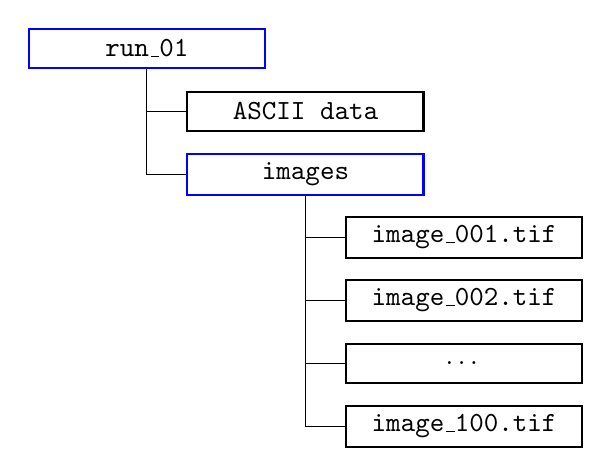
\begin{tikzpicture}
        [ every node/.style = {draw=black,thick,anchor=west,minimum width=3cm,
                               minimum height=0.5cm},
          directory node/.style = {draw=blue},
          grow via three points={ one child at (0.5,-0.8) and two children at
          (0.5,-0.8) and (0.5,-1.6)},
          edge from parent path = { (\tikzparentnode.south) |- (\tikzchildnode.west)}]
        \node[directory node]{{\tt run\_01}}
        child { node {{\tt ASCII data}}}
        child { node [directory node] {{\tt images}} 
            child{ node {{\tt image\_001.tif}}}
            child{ node {{\tt image\_002.tif}}}
            child{ node {\dots}}
            child{ node {{\tt image\_100.tif}}}
        }
        child [missing] {}
        child [missing] {}
        child [missing] {}
        child [missing] {};
    \end{tikzpicture}
    %%\resizebox{\linewidth}{!}{\includegraphics{pics/old_fstree.pdf}}
    \end{minipage}
    \hfill
    \begin{minipage}[c]{0.48\linewidth}
    \caption{{\small A typical directory structure used at todays synchrotron
    experiments. Scalar data is stored in a single ASCII file while detector
    data is stored as individual image files in a separate directory.}}
    \label{fig:nxintro:old_fstree}
    \end{minipage}
\end{figure}

Nexus is a binary file format which attempts to solve all of these problems.
Nexus can keep scalar and multidimensional data within a single file and allows
to organize data in trees. Additional attributes can be attached to each object
in a file storing metadata which might be required for later analysis of the
data. It must be noted that Nexus is not a physical file format itself. It is
rather a set of rules how data must be organized within a particular format in
order to become a valid Nexus file. Currently the following physical file
formats are supported by the original Nexus API
\begin{itemize}
\item XML -- currently only used for file structure validation
\item HDF4 -- for historical reasons, should not be used for new data
\item HDF5 -- the current standard storage backend for Nexus files. 
\end{itemize}
One of the aims of \libpniio\ is to provide an abstraction layer between the
user and the storage backend. As \libpniio\ currently supports only HDF5 this is
rather artificial. However, \libpniio\ provides the architecture to include
other file formats to be used with Nexus too. 
There has been a lot of confusion what physical file format Nexus files are.
Many users think that Nexus has its own phyisical file format. This is in fact
not true. Just to avoid any further confusion fo the reader let me make this
clear once and for all
\begin{quote}
{\huge
{\color{red}Every Nexus file written by \libpniio\ is also a valid HDF5 file!}
\todo[caption={fix quote},inline]{This quote needs better formating. Maybe the
text should go into a box and the margins to the surrounding text must be
bigger}
}
\end{quote}

%%%===========================================================================
\section{The Nexus layer model}

\begin{figure}[tb]
    \centering
    \begin{minipage}[c]{0.5\linewidth}
    \centering
    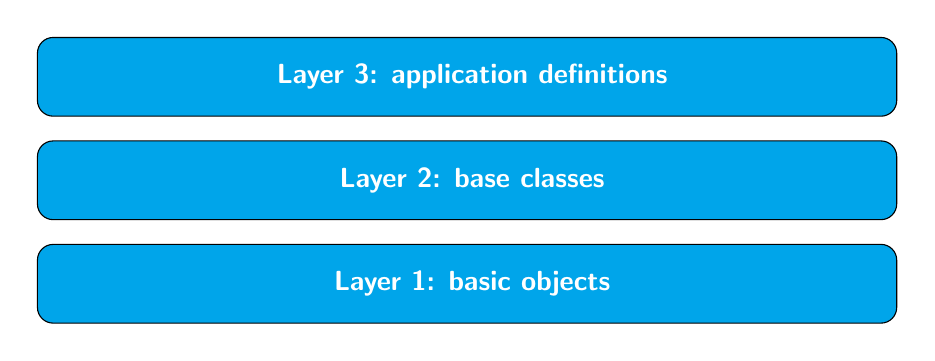
\begin{tikzpicture}
       [layer/.style={fill=desycyan,shape=rectangle,draw=black,
                      minimum width=0.9\linewidth,
                      minimum height=1cm,
                      text=desywhite,align=left,
                      rounded corners=2mm}]
       \matrix[row sep=0.3cm]{
        \node [layer] { \textsf{\textbf{ Layer 3: application definitions}}}; \\
        \node [layer] { \textsf{\textbf{ Layer 2: base classes}}}; \\
        \node [layer] { \textsf{\textbf{ Layer 1: basic objects}}}; \\
        };
    \end{tikzpicture}
    \end{minipage}
    \hfill
    \begin{minipage}[c]{0.45\linewidth}
    \caption{{\small Nexus can be considered to consist of three layers where
    each layer represents a particular level of abstraction.}}
    \label{fig:nxintro:layers}
    \end{minipage}
\end{figure}

\subsection{Layer 1 objects}

\begin{figure}[tb]
    \centering
    \begin{minipage}[c]{0.4\linewidth}
    \centering
    \missingfigure{Need a figure for the layer1}
    %%\resizebox{\linewidth}{!}{\includegraphics{pics/layer1.pdf}}
    \end{minipage}
    \hspace{0.05\linewidth}
    \begin{minipage}[c]{0.5\linewidth}
    \caption{{\small The basic objects of the first layer in the Nexus object
    model.}}
    \label{fig:nxintro:layer1}
    \end{minipage}
\end{figure}

\subsection{Layer 2 objects}

\subsection{Layer 3 objects}

\FloatBarrier

\chapter{Addressing Nexus object - the Nexus path}
%%% describing how to address Nexus objects

\FloatBarrier

\chapter{Basic usage of \libpniio}
%%%describing the basic usage

This chapter deals with the basic interface provided by the layer 1 types
implemented in \libpniio. All types concerning Nexus reside in one of the
namespaces embedded in {\tt pni::io::nx}. The namespaces below this one 
indicate either a particular storage backend (currently only HDF5 is
implemented).

To use the Nexus part of the library just add 
\begin{minted}{cpp}
#include <pni/io/nx/nx.hpp>
\end{minted}
to your source file. 

%%%===========================================================================
\section{Dealing with files}
The most fundamental thing one wants to do is to create, open, and close files. 
A typical usage pattern for a file object would look like this
\begin{minted}{cpp}
#include <pni/io/nx/nx.hpp>

using namespace pni::io::nx;

int main(int argc,char **argv)
{
    h5::nxfile file = h5::nxfile::create_file("test.nxs");
    //... code omitted ...
    file.close();

    return 0;
}
\end{minted}
To create the file we use the {\tt create\_file} static member method of the
{\tt nxfile} class. The available signatures for this function are
\begin{minted}{cpp}
create_file(const string &n,bool ow=false, ssize_t ssize = 0);
create_file(const string &n,bool ow);
create_file(const string &n,ssize_t ssize);
\end{minted}
\todo{Add the missing create\_file signatures to the library}
The arguments have the following meaning
\begin{center}
\begin{tabular}{l|l}
argument & description \\
\hline\hline
{\tt const string \&n} & name of the file \\
\hline
{\tt bool ow} & overwrite an existing file \\
\hline
{\tt ssize\_t sszie} & split size \\
\hline
\end{tabular}
\end{center}
It is important to note the last argument {\tt ssize}. If this argument is
passed and not equal $0$ the HDF5 backend will use the split-driver to write the
data. In this case the file will be split into individual files of size {\tt
ssize} (in MByte). This requires the file name to be a valid C format string
containing an integer index as shown in the next example
\begin{minted}{cpp}
h5::nxfile file = h5::nxfile::create_file("test.%04i.nxs",1024);
\end{minted}
Here the split driver will produced files of $1$GByte size with file names
\begin{minted}{bash}
test.0001.nxs
test.0002.nxs
test.0003.nxs
...
\end{minted}
If a file already exist the {\tt open\_file} static member function of the {\tt
nxfile} should be used. 
Its signature is rather simple 
\begin{minted}{cpp}
open_file(const string &n,bool ro=true)
\end{minted}
where the first argument is again the name of the file to open. The second
optional argument determines whether the file will be opened read-only (the
default) or in read-write mode. 

The file type provides some more methods which should be mentioned here briefly 
\begin{center}
\begin{tabular}{l|l}
method & description\\
\hline\hline
{\tt flush()} & call this method after writing data to ensure that it is written
to disk \\
\hline
{\tt is\_valid()} & return true if the file is valid \\
\hline
{\tt close()} & close a file \\
\hline
{\tt is\_readonly()} & returns true if the file was opened in read-only mode \\
\hline
{\tt root()} & return the root group of the file \\
\hline
\end{tabular}
\end{center}
There are two important remarks to make about files. The first concerns the {\tt
close()} method. It is usually not necessary to call this method explicitly as
the file will be closed automatically when it looses scope. 
The second bears the {\tt flush()} method. This is a rather useful method and
should be called anytime a particular amount of data which can be considered
consistent has been submitted to the file for writing. The {\tt flush()} method 
tells the operating system to take over and write the data.


%%%===========================================================================
\section{Working with groups}

%%%===========================================================================
\section{Working with fields}

%%%===========================================================================
\section{Iterating groups}

%%%===========================================================================
\section{Working with attributes}


\FloatBarrier

\chapter{Using algorithms}
\FloatBarrier

\chapter{Nexus and XML}
%%%documentation concerning the XML functions

As Nexus organizes data objects in a tree like manner, XML is the obvious ASCII
representation for a Nexus file.
\libpniio\ thus provides a small but powerful set of functions to read and write 
Nexus data objects from and to XML files. The framework is based on the 
\cpp{boost::property\_tree} library. 
There are several use cases which should be discussed briefly in 

%%%---------------------------------------------------------------------------
\section{Use cases}\label{sec:xml:usecases}

XML is a powerful and mature technology for representing structured data in 
ASCII. Though it has received some competitors like JSON, when it comes to 
complex structures XML is still the tool of choice\footnote{In fact, JSON
becomes quickly virtually unreadable if the structure becomes too deeply
nested.}
In this section some use cases for Nexus and XML will be presented. 

\subsection{Standard compliance verification of a file}

An always recurring request is the possibility to check a Nexus file with
respect to its compliance to the current standard. As the Nexus standard 
itself is defined in XML it would be reasonable to create an XML representation
of the file to check and use one of the available XML validation tools to 
verify the compliance of the file towards a particular standard. 
Using the XML representation of the file instead of the file directly has 
several advantages 
\begin{itemize}
\item being rather small, the XML representation can also be transfered 
over the network using a remote service for validation
\item it is at least in principle human readable 
\item many of the required tools already exist. 
\end{itemize}
On step in this entire process is to convert a Nexus file to its ASCII XML 
representation.

\subsection{Generating Nexus structures from XML}

The structure of a Nexus file can become rather complex. In a rather complex 
environment like at a synchrotron beamline it would be naive to use static 
code to create the file. A more feasible approach would be to implement 
generic code which generates the structure of a file from an XML template. 
The template could be generated either manually by the user or by means 
of another program written in whatever language is reasonable for this purpose. 

\subsection{Metadata ingestion of a file}

In some situations a $3$rd party may needs to process some of the metadata 
stored in the file while not having access to the file. One possible application
would be a data catalogue. Instead of making the file available the XML dump 
of the Nexus file could be sent to the system while moving the Nexus file 
to its final location on the storage system.

%%%---------------------------------------------------------------------------
\section{Nexus objects from XML}\label{sec:xml::nxtoxml}

%%%---------------------------------------------------------------------------
\section{XML from Nexus objects}\label{sec:xml::xmltonx}

The work horse for Nexus to XML conversion is the \cpp{nexus\_to\_xml} function
template. The most probably simplest use case is demonstrated in the next
example 
\begin{cppcode}
#include <pni/io/nx/nx.hpp>
#include <pni/io/nx/xml.hpp>

using namespace pni::io::nx;

int main(int argc,char **argv)
{
    h5::nxfile f = ....;
    h5::nxgroup root = f.root();

    xml::node root_node;
    xml::nexus_to_xml(root,root_node);
    std::cout<<root_node<<std::endl;

    return 0;
}
\end{cppcode}
Here, the entire structure of the Nexus file is stored below the XML root node 
which is at the end dumped to standard output.
This simple example already raises an important question: how to deal with the
data stored in the Nexus file. As Nexus files can be used to store large amounts
of data it would not be wise to convert all this data to ASCII (think about a 3D
image stack stored in the file). However, some data might be required. 
The \cpp{nexus\_to\_xml} template thus provides a third optional argument which 
is a predicate function which decides for which field or attribute data will be
written to the file. 
The signature of the predicate is 
\begin{minted}[fontsize=\tiny]{cpp}
template<
         typename GTYPE,
         typename FTYPE,
         typename ATYPE
        >
bool predicate(const nxobject<GTYPE,FTYPE,ATYPE> &o);
\end{minted}
The function returns \cpp{true} if the data of a particular object should be 
included in the XML output. 
It is wise to not make this function to specific. Thus, the name of a field 
is not a good criterion for deciding whether or not to write data. 
A much better approach is to check for certain properties of an object. 
For the previous example a possible predicate could look like this
\begin{cppcode}
//code omitted 
bool write_predicate(const h5::nxobject &o)
{
    if(is_field(o) || is_attribute(o))
    {
       return size(o)==1;
    }
    else 
        return false;
}

int main(int argc,char **argv)
{
    //code omitted 
    xml::nexus_to_xml(root,root_node,write_predicate);

    //code omitted
    return 0;
}
\end{cppcode}
This predicate determines that only the data from fields and attributes 
is written to the XML tree if their size is equal to $1$ (in other words -- only
scalars are written to the file). 
Such an approach keeps the resulting XML document small while using a rather 
general predicate which would match quite a lot of use cases.


\FloatBarrier

\appendix
\chapter{Parsing ASCII data}\label{appendix:parsers}

In times of binary data formats like Nexus it seems anachronistic to devote an
entire chapter of the appendix to the problem of ASCII parsing. However, 
ther are several good reasons why one should care about correctly reading 
ASCII data (in particular numbers)
\begin{enumerate}
\item for historical reasons there is a lot of legacy ASCII data out there which
may should be processed -- for this reason alone it is necessary to deal with
ASCII data in a reasonable way.
\item uses still provided input to programs via ASCII files (for instance using
XML) or via the command line -- in both cases the program has to process these
files correctly. 
\item even input fields in GUI toolkits typically return the data entered by 
the user as an characater string which must be parsed in order to obtain a 
numerical value.
\end{enumerate}

One crucial aspect when processing ASCII data is number parsing.
This chapter will describe in more detail the parser framework provided by 
\libpniio. 

All parsers basically utilize two exceptions to denote errors
\begin{description}
\item[\texttt{parser\_error}] which is thrown in situations where the ASCII 
representation is malformed, or
\item[\texttt{range\_error}] which is thrown when the ASCII string is well 
formatted but the numeric range represented by the number exceeds the 
target type {\bf not yet implemented}
\end{description}
This information should be sufficient to recognize the error in the input data. 
Before discussing the individual functions and types provided by \libpniio\ 
for parsing ASCII a thorough discussion of the ASCII representations of 
the primitive data types will be made.

%%----------------------------------------------------------------------------
\section{ASCII representations of primitive data types}

\subsection{Integers and floating point numbers}
The ASCII representations of integer and floating point numbers follow the 
C++ standard conventions and will not be discussed here in greater detail.

\subsection{Complex numbers}

Complex numbers can be represented in two forms: as real and imaginary part 
or as imaginary part only. A real-part only representation is not possible 
as such a number would be indistinguishable from a simple floating point type. 
The full representation (real and imaginary part) looks somehow like this
\begin{align}
A \pm K B
\end{align}
where $A$ and $B$ are denoting the real and imaginary part respectively. 
$K$ is the symbol which denotes the complex unit $\sqrt{-1}$. This can be either
$i$, $j$, or $I$. To given an example 
\begin{verbatim}
1.2+j3.4
\end{verbatim}
would be a valid complex number while
\begin{verbatim}
1.2+J2.4
\end{verbatim}
not. It is important to not that the sign between the real- and imaginary-part 
must not be surrounded by blanks. Furthermore, the imaginary part must not have
an extra leading sign as its sign is already determined by the sign between
real- and imaginary part. 
A imaginary-part only number would look like this
\begin{verbatim}
+i3
\end{verbatim}
where the sign in front of the complex unit is optional and could have been 
omitted in this particular case 
\begin{verbatim}
i3
\end{verbatim}

\subsection{Boolean values}

The two boolean values \cpp{true} and \cpp{false} are represented exactly in
this way as ASCII strings. Be aware that the syntax is case sensitive. Thus 
\cpp{True} or \cpp{False} would cause a \cpp{parser\_error}.

%%----------------------------------------------------------------------------
\section{Parser rules}




\FloatBarrier


%\bibliography{libpniio_ug}

\end{document}
